\documentclass{book}

	\usepackage[dutch]{babel}
	\usepackage{lipsum}
    \usepackage{hyperref}
	\usepackage{booktabs}
    \usepackage[utf8]{inputenc}
    \usepackage[a4paper,margin=2.5cm]{geometry}
    \usepackage{cite}
    \usepackage{multirow}
   	\usepackage{setspace}
    \usepackage[parfill]{parskip}
    \usepackage{graphicx}
    \usepackage[margin=1cm,font=small,labelfont=bf]{caption}

	\newcommand{\CaptionFontSize}{\small}


\begin{document}

\chapter*{Dankwoord}
Vergeet in het dankwoord niet je promotor/co-promotor en begeleider te bedanken. Denk ook aan eventuele externe begeleiders !

\chapter*{Samenvatting}
Dit is, zoals de titel zegt, een samenvatting van de tekst. Zorg dat deze begrijpelijk is zonder dat je de tekst gelezen hebt. Niet teveel technische termen dus; wees volledig maar beknopt. Tracht een goed overzicht te geven van je eigen bijdrage. Dit hoofdstuk mag uiteraard ook geen informatie bevatten die nergens in de tekst terugkomt (geen enkel sectie/hoofdstuk in de tekst mag dus terugverwijzen naar de samenvatting).

\lipsum[1]{}

\tableofcontents

\chapter{Inleiding}
\label{Inleiding}

Het eerste hoofdstuk begint met een situering van de tekst/het onderwerp van de proef in de brede context. Formulier hier ook je onderzoeksvraag (ook belangrijk voor je poster !)

\section{NIET doen}

\begin{itemize}
\item Het is expliciet NIET toegelaten lijsten van figuren, tabellen, code samples enz in de tekst op te nemen. Enkel de secties die in dit document vermeld zijn (samenvatting/dankwoord/inhoudsopgave/eigenlijke tekst/conclusies) mogen erin staan.
\item Belangrijk ! Maak geen secties met minder dan 5 zinnen; elk onderdeel moet een \textbf{substantieel} stuk tekst bevatten.
\item Zorg dat je geen 'lonely' sections hebt. Dus bv geen 3.2.1 als er geen 3.2.2 is. 
\end{itemize}

\section{WEL doen}
\begin{itemize}
\item Je mag 3 niveau's diep gaan in je tekst, indien het er meer zouden zijn moet je de structuur onder handen nemen. 
\item Verzorg je taalgebruik (denk aan dt-fouten, consistent gebruik van huidige/verleden tijd enz)
\item Referenties voeg je in via bibtex. Het referentieformaat mag je zelf kiezen, maar onze voorkeur gaat uit naar een type dat het publicatiejaar integreert in de reference (bv iets als [JANSSEN03] en niet louter een abstract nummertje). De bibliografie is het laatste stuk van je tekst.

\end{itemize}


\chapter{Tweede hoofdstuk}
\label{tweede_hs}

Schrijf hier de inleidende tekst voor hoofdstuk 2.


\section{Voorbeelden van tabellen}

Zorg dat je tabellen verzorgd zijn. Verticale lijnen vermijden we ! Voor meer info kan je ook kijken op \url{https://www.inf.ethz.ch/personal/markusp/teaching/guides/guide-tables.pdf}

  \begin{tabular}{llr}
  \toprule
  First name & Last Name & Grade \\
  \midrule
  John & Doe & $7.5$ \\
  Richard & Miles & $2$ \\
  \bottomrule
  \end{tabular}

  \vspace{0.5cm}

  \begin{tabular}{llr}  
    \toprule
    \multicolumn{2}{c}{Item} \\
    \cmidrule(r){1-2}
    Animal    & Description & Price (\$) \\
    \midrule
    Gnat      & per gram    & 13.65      \\
          &    each     & 0.01       \\
    Gnu       & stuffed     & 92.50      \\
    Emu       & stuffed     & 33.33      \\
    Armadillo & frozen      & 8.99       \\
    \bottomrule
  \end{tabular}

\section{Figuren}

Indien je figuren invoegt in het document, zorg dan dat ze van behoorlijke kwaliteit zijn (geen upscaling van low quality JPEGs bijvoorbeeld). Indien je kopieert van een bestaande bron, zet er een duidelijke en expliciete bronvermelding bij. Schema's enz maak je bij voorkeur zelf ipv te knippen/plakken. De caption onder de figuur moet op zichzelf leesbaar/begrijpbaar zijn. Dus niet gewoon `screenshot' of `grafiek van de bandbreedte' vermelden. 

\begin{figure}
\centering\CaptionFontSize
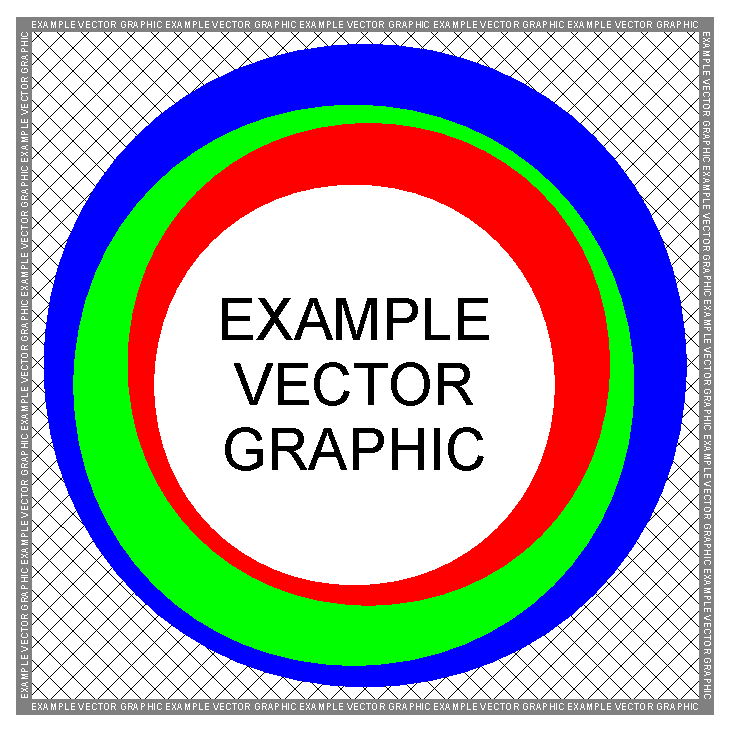
\includegraphics[height=15em]
{fig1}
\caption[]
{Hier komt de volledige caption van de figuur.}
\label{Figure:ChapAbbr:FigureExampleA}
\end{figure}


\chapter{Voorbeeldtekst}
\label{Tekst}

\lipsum{}
\section{Sectie}
\lipsum{}
\subsection{Subsectie}
\lipsum{}
\subsection{Subsectie}
\lipsum{}
\section{Sectie}
\lipsum{}


\chapter{Conclusies}
\label{Conclusies}

Hier schrijf je de conclusies. Belangrijk : dit is GEEN samenvatting van de tekst. In dit onderdeel beschrijf je je bevindingen en een persoonlijke reflectie op het onderwerp en het leerproces dat je doorlopen hebt bij het implementeren/schrijven van de bachelorproef. 10 Regels volstaan hier niet! Het moet een samenhangend stuk tekst zijn met een belangrijke boodschap voor de lezer. Je mag/moet kritisch staan ten opzichte van de opdracht en de behaalde resultaten.


\end{document}